\documentclass[preprint]{sigplanconf}

% The following \documentclass options may be useful:
% preprint      Remove this option only once the paper is in final form.

\usepackage{amsmath}
\usepackage{graphicx}
\usepackage{hyperref}
\usepackage{url}

\newcommand{\ALGOL}{A\textsc{LGOL}}
\newcommand{\MATLAB}{\textsc{MATLAB}}
\newcommand{\Mathematica}{\textit{Mathematica}}
\newcommand{\code}[1]{\texttt{#1}}

\begin{document}

\special{papersize=8.5in,11in}
\setlength{\pdfpageheight}{\paperheight}
\setlength{\pdfpagewidth}{\paperwidth}

\conferenceinfo{ARRAY '14}{June 15, 2014, Edinburgh, UK}
\copyrightyear{2014} 
%\copyrightdata{978-1-nnnn-nnnn-n/yy/mm} 
%\doi{nnnnnnn.nnnnnnn}

% Uncomment one of the following two, if you are not going for the 
% traditional copyright transfer agreement.

%\exclusivelicense                % ACM gets exclusive license to publish, 
                                  % you retain copyright

\permissiontopublish             % ACM gets nonexclusive license to publish
                                  % (paid open-access papers, 
                                  % short abstracts)

\titlebanner{Array Operators Using Multiple Dispatch}    % These are ignored unless
\preprintfooter{Array Operators Using Multiple Dispatch} % 'preprint' option specified.

% \title{Array implementations in Julia}
% \subtitle{Implementing arrays in a way that is amenable to compiler analysis}

%\title{Array Operators Using Multiple Dispatch}
%\subt
\title{ A design methodology for array implementations in dynamic languages }

\authorinfo{Jeff Bezanson \and Jiahao Chen \and Keno Fischer \and Alan Edelman}
           {MIT Computer Science and Artificial Intelligence Laboratory}
           {\{ bezanson, jiahao, kfischer, edelman \}@csail.mit.edu}
           
       \subtitle{   [Add Stefan and Viral??] }

%TODO Get Dahua to sign on as coauthor
%\authorinfo{Dahua Lin}
%           {Toyota Technological Institute at Chicago}
%           {dhlin@ttic.edu}

\maketitle

\begin{abstract}

Arrays, the most basic of data structures, tends to be built in to a language early
either in the compiler or a large low-level library. 
More recent developments
beg for more flexibility and generality, as
modern array programming systems are typically integrated with object-oriented
languages.  A consequence of the traditional approach is that the array data type is difficult to
modify or extend, and is even unnecessarily more difficult to implement.

% ??  [The below delays the good point]
%Arguably, efficient
%and flexible n-d arrays are one of the more difficult datatypes to implement
% at the library level.

In this work, we present a new approach, developed as part of 
the Julia language project, where the object system is used to define the behaviors
of  \framebox{  {\bf key array operators} } \marginpar{Which operators?  Which functionality?  reshape? indexing? others? too vague}  --- not just to organize the 
\framebox{  {\bf functionality} } into
classes.
The combination of flexible multi-method
signatures and dataflow type inference yields a novel trade-off between
flexibility and compiler analysis.

\framebox{The words ``multiple dispatch'', should appear in the abstract?}
\end{abstract}

%\category{CR-number}{subcategory}{third-level}

\keywords
Julia, multiple dispatch, type inference, array indexing, static analysis,
dynamic dispatch

\section{Introduction}

\begin{quotation}
``Unfortunately, it is very difficult for a designer to select in advance all
the abstractions which the users of his language might need. If a language is
to be used at all, it is likely to be used to solve problems which its
designer did not envision, and for which abstractions embedded in the language
are not sufficient.'' - Ref. \cite{Liskov:1974pb}
\end{quotation}

Arrays are an essential data type for many programming languages for
organizing multiple elements of the same type. (In fact, they are the oldest
data structures to be conceived of and implemented on computers.
\cite{Zuse:1948ua, Rojas:2000pk, Backus:1956pr}.) Nevertheless, arrays are a
commonality amongst languages that nonetheless are divided in terms of
implementation of underlying data structures.

%TODO Cite Knuth TAoCP vol 1, which had something interesting to say here
%about implementations.

Unless otherwise stated, an $n$-array (array of rank $n$, or simply `array')
is considered in this paper to be implemented as a tuple of a memory buffer
and shape information, with $n$ being the rank of the array. Key to
implementing array semantics is the conversion of indices of one or more array
elements into memory addresses where the elements are located. 1-arrays are
available in most programming languages, since the conversion of a single
index into a memory offset is simple and straightforward. However, the general
$n$-arrays which are often required for technical computing pose significantly
greater challenges for authoring libraries, be they in the base library of a
programming language, or popular third-party libraries.

\section{Implementation challenges of $n$-arrays}

Three specific challenges can be identified:

\begin{enumerate}

\item{\bf Efficiency:} Code that operates on the dimension sizes needs to be
highly efficient. Typically the overhead of a loop is unacceptable, and such
code needs to be fully unrolled. Efficiency begs for static analysis which
would enable compile-time optimizations such as constant subexpression
elimination of indexing computations and loop fusion/reordering of array
traversals.

\item{\bf Dynamic applications:} Some applications require arrays of dynamic
ranks, i.e. the ranks are only known at runtime. To support such applications,
array implementations cannot use data structures that fit in a constant amount
of memory. Dynamic properties call for runtime flexibility.

\item {\bf Dimension specialization:} Programs may wish to treat arrays with
different numbers of dimensions very differently. A vector---an intrinsically
one-dimensional object---is conceptually very different from an $N\times1$
matrix, which is intrinsically two-dimensional. For example, it may be
important in certain applications to distinguish between vector norms and
certain types of matrix norms. Also, many linear algebraic computations like
the singular value decomposition make sense only for matrices, not vectors.
These differences in object semantics and behavior make the number of
dimensions a crucial part of program semantics and thus cannot be merely a
compiler implementation detail. Even though it is possible to construct an
isomorphism between column vectors and $N\times1$ matrices, semantic
differences preclude a genuine ``is-a'' relationship, and hence results in a
violation of the Liskov substitution principle \cite{Liskov:1987da}. We can
think of this situation as the linear algebraic counterpart to the canonical
circle-ellipse problem \cite{Halbert:1987ut}.

Dimension specialization suggests that dimensionality should be part of the
type system, but partly determined at run time (for example, via virtual
method dispatch).

\end{enumerate}

These three factors together call for both static and dynamic analyses of
program semantics involving arrays. Hence, implementations of programming
languages must choose a compromise between dividing the work between compile-
time and runtime.

\subsection{Implementation strategies for arrays}

Some of the common strategies are

\begin{enumerate}

\item {\bf Rank limits:} Some programming languages or their implementations
impose a strict limit on the maximal rank of $n$-arrays.

Fortran is perhaps the most famous example in this category: the maximal rank
was 3 in FORTRAN I \cite{Backus:1957fa}, was increased to 7 in Fortran 77,
and later to 15 in Fortran 2008. Furthermore, only static arrays were allowed
until the \code{ALLOCATABLE} keyword was introduced in Fortran 90. The
traversal semantics were hard-coded into the compiler \cite[pp.~10--
11]{Backus:1956pr}, and index-to-offset computations lead to nontrivial
compiler design challenges for efficient implementation, such as common
subexpression elimination for computing strides, and loop fusion for certain
types of array traversal \cite{Busam:1969oe}.

%XXX Fortran started with only arrays; objects were added later: Arrays were
%the only compound type supported by Fortran. In Fortran however, arrays were
%a fundamental part of the language from the very beginning, whereas objects
%were not introduced until the advent of Object-Oriented Fortran and Fortran
%2003.

%TODO examples of systems limited to n==3
%TODO Java?

The advantage of imposing rank limits is that specialized implementations for
each rank $n$ can be written out in full. The disadvantage, of course, is that
program expressibility is limited and it is challenging to write libraries for
general $n$-arrays in these languages.

\item {\bf Static flexibility:} Some systems provide flexibility only at
compile time, for example a template library where the rank must be statically
known.

\ALGOL{} 60 is the oldest language in this category, supporting general
$n$-arrays that were even allowed to change size at runtime. Implementing
these array semantics posed numerous challenges for compiler writers of the
time \cite{Randell:1964a6}. Among the innovations they produced were the
notions of \textit{dope vector} \cite{Sattley:1960as, Sattley:1961as}, which
contained the size and lower bound of each dimension, and the closely related
\textit{storage mapping function} \cite[pp.~80--87]{Randell:1964a6}. These
innovations are the first documented examples of abstracting out shape
information from arrays.

C is another famous example in this category. Strictly speaking, C supports
only 1-arrays; nevertheless, nested arrays of arrays allow C programs to work
with $n$-arrays of fixed rank. Thanks to the equivalence of pointer arithmetic
and array indexing in C \cite[pp.~93--96]{Kernigham:1978cp}, both static and
dynamic arrays can support the same \code{A[i][j]} indexing semantics.

%TODO something about the n-dimensional circle-ellipse problem for arrays of arrays?

%XXX In some sense, C does not have a disjunction between arrays and other
% objects. In C, objects and arrays can only be accessed semantically with
% pointers. To the extent that C has a minimalist approach to both objects and
% arrays, they are not disjoint.

%XXX Unused C++ material.

% You can try to use the object system in C++ to implement arrays, but it's a
% disaster.
%
% C++ does not introduce a fundamentally new way to handle arrays. One might
% argue that dynamic and static arrays are implemented by the \code{std::vector}
% and \code{std::array} classes of the C++ Standard Library. However, the
% semantics are hard coded for one dimension only. Furthermore, directly
% indexing a vector \code{a[i]} is not required to incur a bounds check (such
% behavior is undefined by the standard), but only with the more cumbersome
% syntax \code{a.at(i)}, which then throws an \code{std::out\_of\_range}
% exception if \code{i} is out of bounds. In principle, a container resembling
% multidimensional arrays can be created by chaining these classes together,
% forming syntactically awkward constructions like
% \code{std::vector<std::vector<...>>}. However, this strictly speaking is not
% an array data structure if one consider a contiguous memory store to be one of
% the defining features of arrays, as there is no guarantee that C++ will
% allocate memory in this fashion. Additionally, the distinction made between
% \code{vector}s and \code{array}s in principle could lead to very strange
% constructs that are static in some dimensions but dynamic in others, e.g. in
% the chain \code{std::vector<std::array<...>>}. Furthermore such nested constructs
% do not interoperate well with other parts of the C++ standard library such as
% iterators or even \code{max\_element}, thus limiting their usefulness
% \cite{Bavestrelli:2000ct}.
%
% In practice, the high cost of iterative containers means that such constructs
% are not widely used.

Another prominent example is C++. C++ is sufficiently powerful to allow the
implementation of $n$-arrays in fast, performant libraries. Notable examples
include \code{Blitz++} \cite{Veldhuizen:1998ab} or \code{Boost.MultiArray}
\cite{Garcia:2005ma}, which implement $n$-arrays using C++ expression
templates. \code{Boost.MultiArray}s are defined not just by memory store and
shape, but also index bases (first index in each dimension) and strides
\cite{Garcia:2005ma}. In particular, the stride specification allows for
arrays to be stored in row-major or column-major order (or their
multidimensional generalizations) as desired.

Nevertheless, template metaprograms are nonetheless notoriously difficult to
implement and comprehend. While $n$-arrays can be implemented compactly using
recursive template metaprograms \cite{Bavestrelli:2000ct}, exploiting
recurrences between $n$-arrays and $(n-1)$-arrays, production quality
libraries avoid explicit recurrences, implementing instead a great many
special-cased implementations of $n$-arrays to ensure that C++ compilers
unroll loops fully to achieve maximal performance \cite{Garcia:2005ma}. Also,
C++'s semantics for \code{operator[]} means that indexing must recurse from
leftmost to rightmost index. Furthermore C++ expression templates make liberal
use of the static (compile-time) semantics which are not accessible
dynamically (at runtime). Also you have handle dimensions one at a time.

%TODO something about how this implements extra work for playing nice with STL
%features like std::iterators?

%TODO: insert example of limited power of C++ array libraries

%TODO Something about transposition costs regarding implementation?

Haskell is another useful example. A purely functional like Haskell, which
disallows imperative constructs like loops, arguably forces programmers to
identify abstractions. With fewer options to implement semantics, semantics is
more intimately tied to types. You can see this in the Repa (Regular Parallel
Arrays) library. One key abstraction is the \code{Shape} class, which enables
dispatch on the index-to-offset mapping function \cite{Keller:2010rs}. This
allows for in-memory representations of transposed arrays, simply by changing
the \code{Shape} class to redefine the memory striding rules
\cite{Keller:2010rs}.

Repa still has some issues though. There is an intrinsic recurrence over array
rank that is reminiscent of the C++ expression template approach
\cite{Keller:2010rs}. For example, reductions like \code{Sum} are only defined
over the last index \cite{Keller:2010rs}. In principle, a generalized
\code{Sum} over an arbitrary index can be composed as \code{Sum} with pre- and
post-permutations to swap the desired index with the last index. However,
this is semantically more work and furthermore isn't guaranteed to produce a
good memory traversal pattern. Similarly, operations over more than one
dimension are implemented recursively over the dimensions, which means that
the compiler has to make the difficult decision whether or not to unroll the
recursion \cite{Lippmeier:2011ep}. Manual unrolling is of course a possibility
but has the cost of introducing repetition in the code
\cite{Lippmeier:2012gp}.

%TODO A static # of dimensions is probably sufficient for
% most applications, but there is a large cliff where everything
% changes if your code is more dynamic

\item {\bf Full flexibility:} Some systems choose flexibility, accepting that
that most or all operations will be dynamically dispatched. Mathematica{} and
\MATLAB{} and Python/Numpy are prominent examples in this category.

\Mathematica{} implements $n$-arrays using nested lists of expressions
\cite{mathematica:nl, mathematica:int}, with the \code{[[]]} (\code{Part})
operator playing the role of array indexing. The flexibility engendered by the
pattern matching semantics of \Mathematica, however, comes at a price. First,
arrays, which are implemented as lists, are no different from ordinary lists.
\Mathematica{} arrays are therefore leaky data abstractions. For example, it
is possible to ``index'' an array with more indices than its rank; the extra
indices would simply traverse into the expression contained within the matrix
element. For example, \code{Array[f, {3, 4}][[3, 2]]} returns \code{f[3,2]},
whilst \code{Array[f, {3, 4}][[3, 2, 1]]} returns \code{3}. Thus the semantics
of the \code{Part} symbol is more general than pure array indexing and allows
for violations of the array data abstraction, which may come as a surprise to
users. Additionally, the flexibility of the \Mathematica{} language limits the
ability of static analyses (based on a finite-height partial order over
patterns) can discover about any given \Mathematica{} program.

\MATLAB's flexibility is also potentially problematic, since user-defined
classes can behave arbitrarily differently. Since \MATLAB{} arrays are not
defined in terms of its object system, special care must be taken for arrays
of user-defined classes to have the same semantic behavior as arrays of built-
in types.

% Jeff calls this "just overloading".

\MATLAB's array semantics pose challenges for static compilers, like
automatically enlarging an array when a write occurs to an out-of-bounds
reference. Static compilers essentially had to implement a \MATLAB{} type
system to do type inference and value propagation, thus requiring additional
compiler passes with forward interprocedural flow analysis to check
specifically for array assignments spread over multiple assignment
statements, possible shape and range value changes due to out-of-bounds
indexing, and also the possibility of implicit type promoting resulting from
algebraic operations, e.g. real to complex \cite{Rose:1999tt, Li:2013mf}.
Additionally, type checking was essential to disambiguate \MATLAB{}
expressions like \code{A*B}, which, depending on the dimensions of \code{A} and
\code{B}, could represent a scaling, inner product, outer product, matrix-
matrix multiplication, matrix-vector multiplication \cite{Rose:1999tt}. FALCON
also tries to detect symmetry of matrix (triangular, etc.) and dispatch
appropriate BLAS routines \cite{Rose:1999tt}.

%TODO It's not clear if the matrix symmetry detection is a static analysis or not.

Similar issues also pose challenges for the Octave interpreter \cite{Eaton:2001op}.

%XXX \Mathematica{}
%interprets nested lists of depth $n$ as rank-$n$ multidimensionary arrays
%(which are termed ``tensors'' in \Mathematica), but at the same time
%implicitly assumes the isomorphism between, say, rank-4 arrays and matrices of
%matrices, which \Mathematica{} takes advantage of when displaying results in
%\code{MatrixForm}. For example, the code
%\begin{verbatim}
%Zero[n_] := Table[0, ##] & @@ Table[{2}, {n}]
%\end{verbatim}
%generates the zero array of rank $n$ and size (2,2,\dots,2), which when 
%displayed in \code{MatrixForm} will render as nested matrices and vectors, as 
%demonstrated in Figure~\ref{fig:mathematica}.
%
%\begin{figure}
%  \centering
%  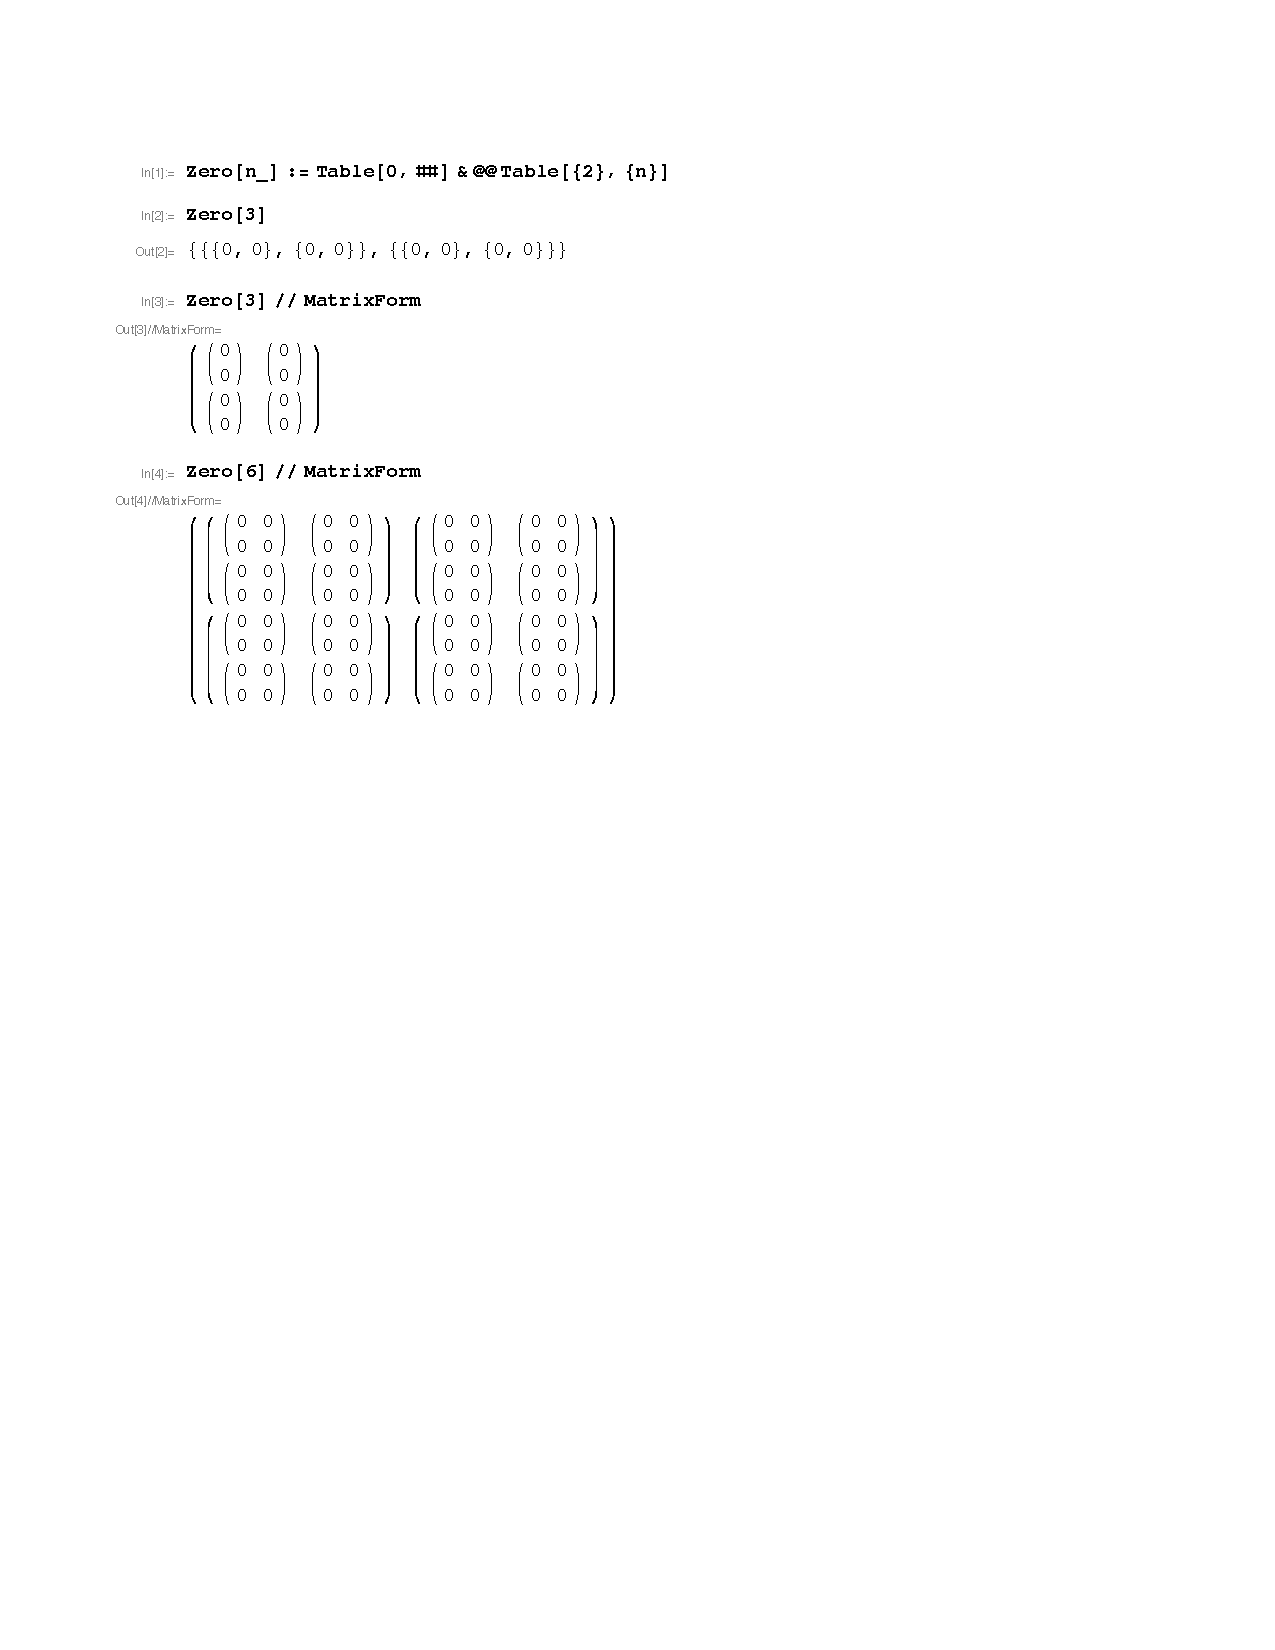
\includegraphics[width=\columnwidth]{fig-mathematica/fig.pdf}
%  \caption{\label{fig:mathematica} Creating and displaying the zero array of
%rank $n$ and size (2,2,\dots,2). ($n=3$ and $n=6$ shown.) \Mathematica's
%\code{MatrixForm} function nests two dimensional structures.}
%\end{figure}

Another example is Python/NumPy in particular.

NumPy arrays are Python objects but the mechanism of the object system don't
play a huge role in defining behavior. Instead, NumPy has its own abstraction
mechanisms implemented with a large C code base for compile-time code
generation and custom runtime dispatch mechanisms. The resulting Python
objects are little more than lookup tables of behaviors, primarily centered
around indexing behavior, and in particular indexing of a single index.

%TODO other languages: R, APL, ZPL?

\end{enumerate}

\subsection{Summary}

Arrays suffer from dearth of abstraction - lots of manual implementation, hand
coded into the compiler, implementation is imposed on users. Oftentimes the
object system is disjoint from the arrays, e.g. R types, because these
subsystems were tacked onto the language at different points in time.

Implementation details: row vs column major, indexing rules, etc., constrain
how users have to deal with stuff.

\section{Array indexing}

Whatever decision is made, rules must be defined for how various operators act
on dimensions. For now we will focus on indexing, since selecting parts of
arrays has particularly rich behavior with respect to dimensionality. For
example, if a single row or column of a matrix is selected, does the result
have one or two dimensions? Array implementations prefer to invoke general
rules to answer such questions. Such a rule might say ``dimensions indexed
with scalars are dropped'', or ``trailing dimensions of size one are
dropped'', or ``the rank of the result is the sum of the ranks of the
indexes'' (as in APL).

%TODO indexing in other languages: C++, Haskell,...

\subsection{Indexing oddities in MATLAB}

Arrays are the most fundamental data type in \MATLAB{}, and all \MATLAB{}
arrays must have at least two dimensions. Consequently, row vectors, column
vectors and scalars are treated as isomorphic to matrices with dimensions
$1\times N$, $N\times1$ and $1\times1$ respectively. This reflects \MATLAB's
original design principle as a ``\textbf{matrix} laboratory".

Not having pure scalars can be mathematically troublesome. For example, the
product $A_{m\times n} \times B_{1\times 1} \times C_{n\times p}$ is invalid
under the ordinary rules of matrix multiplication for $n\ne1$; however,
\MATLAB{} would allow the evaluation of this product by interpreting $B$ as a
scalar which commutes with $A$ and $C$, allowing this product to be evaluated
as the product of the scalar $B_{11}$ and the matrix product $A_{m\times n}
\times C_{n\times p}$.

%TODO Find examples where this kind of interpretation breaks commutativity or
%associativity. Matrices of matrices or matrices of quaternions?

Also, all arrays are treated as if they have an infinite number of trailing
singleton dimensions. This reflects a later design decision in \MATLAB{} to
support multilinear algebra \cite{matlabman:ma, Rose:1999tt}, albeit in a
manner that does not quite mesh with the world of ordinary linear algebra.
This unfortunately clashes with the \textit{linear indexing} rule in \MATLAB{}
that indexing a multidimensional array with a single index automatically
triggers a reshape. For example, for $A_{3\times4}$, there is an ambiguity as
to whether \texttt{A(5)} means \texttt{B=A(:);B(5)} or
\texttt{A(5,1,1,\dots)}, and this ambiguity can only be resolved by performing
a runtime bounds check as a consequence of an arbitrary design decision.

\MATLAB{} also allows indexing with matrices, but they are treated as if they
were flattened for indexing purposes, i.e.
\begin{verbatim}
A(M1, M2, dots) = A(M1(:), M2(:)), dots
\end{verbatim}

There is also something very funky with \MATLAB's cell arrays. You have to
index into them using \texttt{A\{...\}} instead of the usual \texttt{A(...)}.

%TODO Find an example for which this causes problems?

%TODO Problems for static compilers for dynamics languages? Matlab in particular?

\section{Julia Arrays}

Julia uses the object system to implement arrays. Arrays are implemented as
the \code{Array} data type, which is parametric on the \code{Type} of element
it contains, and also its rank (which defaults to 1). Internally,
\code{Array}s are implemented as a pair of (shape, linear data storage) =
metadata of bounded size O(1) + raw data O(N). This basic structure is
sufficient to define the semantics of multidimensional arrays, yet is flexible
to incorporate a wide range of nontrivial design decisions.

One of the core features of Julia is multiple dispatch. Consequently, it is
possible for \code{Array}s to have implementations that afford both generality
and efficiency. The most general \code{Array\{Any\}} is an associative array
implemented as an array of pointers to heap-allocated values. However,
\code{Array}s of native machine types like double precision floating point
numbers (\code{Float64}s) or integers of native machine size (\code{Int}s) can
be implemented to be C/Fortran-compatible. Interestingly,
\code{Array\{Nothing\}} can be implemented with zero storage space at runtime,
since it consists of elements of an immutable type with zero fields, which is
possible because only a single instance of any such type can exist, and hence
need not actually be stored. This allows for some clever tricks like
implementing \code{Set\{T\}} using a \code{Dict\{T,Nothing\}} to avoid paying
any cost for the value array in the \code{Dict}.

Contrast the Julia approach to static compilers for other dynamic languages,
e.g. FALCON (a \MATLAB{} static compiler). The latter use dynamic type
inference used to speed up existing language implementation. Great, but what
you should really do is figure out how to redesign the language given that
technique, to take full advantage of it.

Contrast the Julia approach to the C++ expression template approach. Julia, as
a dynamic language, does not have separate static and dynamic semantics.
Unlike templates, which are effectively a separate language, the single all-
runtime model of Julia is much easier to use and imposes fewer restrictions on
the kind of Julia code that can be written. You can implement a bigger class
of rules in Julia rather than having to special case on the number of
dimensions or be forced to rely on recursive definitions onto subarrays. For
example in Julia you can do `A[I...]` where `I` is a heterogeneous array, and
all the same definitions are still applicable, but you might take a bit of
performance drop.

Contrast the Julia approach to NumPy's. Dynamic dispatch is powerful, but
Julia's approach is much more powerful. We believe that a single powerful
dispatch mechanism can subsume both the compile-time code generation
challenges and custom run-time dynamic dispatch mechanism in NumPy.

Contrast the Julia approach to Haskell/Repa. Statically typed languages tend
to favor recursion down array ranks one at a time, which limit how you can do
operations across multiple dimensions. In Julia we have access to the entire
argument list, which lets you have different mental models and APIs.
Multiple dispatch is also a powerful alternative to the single dispatch
mechanism of Haskell based on function classes and pattern matching, which Repa
uses extensively to implement the many array representations which were
introduced to deal with many different use cases
\cite{Lippmeier:2011ep,Lippmeier:2012gp}.

\subsection{Indexing rules}

Here we consider the indexing rules. How to compute shapes of subarrays. How
to deal with singleton dimensions is but a very special case even though
superficially the rules mention them explicitly.

In Julia, such indexing rules are defined in exactly one place and can be
changed later if so desired.

\subsubsection{The need for flexibility in array indexing rules}

Our goal here is a bit unusual: we are not concerned with which rules might
work best, but merely with how they can be specified, so that domain experts
can experiment.

In fact different domains want different things. E.g. in images, each
dimension might be quite different, e.g. time vs. space vs. color, so you
don't want to drop or rearrange dimensions very often.

In practice we may all have to reach a consensus on what rules to use, but it
should not be enforced upon uses by pure technical implementation convenience.
The point is that in Julia, these are not enforced a priori. Sometimes the
distinctions between the various indexing rules are semantically meaningful
and that's when this flexibility becomes particularly valuable. For example
Tim Holy's image 4-arrays. Quantum mechanics when you average out multiple
indistinguishable particles. $n$-point correlations functions where which $k$
indices you average out defines any number of lower-point $n-k$ point
correlation functions.

\subsection{Ground rules}
Here are our ground rules:

\begin{enumerate}
\item You can't manually implement the behavior inside the compiler
\item The compiler must be able to reasonably understand the program
\item The code must be reasonably easy to write
\end{enumerate}

Instead of the compiler will analyze indexing expressions and determining an answer
using hard-coded logic, we would rather implement the
behavior in libraries, so that different kinds of arrays may be defined, or so
that rules of similar complexity may be defined for other kinds of objects.
But these kinds of rules are unusually difficult to implement in libraries. If
a library writes out its indexing logic using imperative code, the host
language compiler is not likely to be able to analyze it. 

Our dispatch mechanism permits a novel solution. If a multiple dispatch system
supports variadic functions and argument ``splicing'' (the ability to pass a
structure of $n$ values as $n$ separate arguments to a function), then
indexing behavior can be defined as method signatures.

This solution is still a compromise among the factors outlined above, but it
is a new compromise that provides a net-better solution.

%TODO more

\subsection{\texttt{index\_shape}}

Below we define a function \texttt{index\_shape} that computes the shape of a
result array given a series of index arguments. We show three versions, each
implementing a different rule that users in different domains might want:

\begin{verbatim}
# drop dimensions indexed with scalars
index_shape() = ()
index_shape(i::Real, I...) = index_shape(I...)
index_shape(i, I...) = tuple(length(i), index_shape(I...)...)
\end{verbatim}

\begin{verbatim}
# drop trailing dimensions indexed with scalars
index_shape(i::Real...) = ()
index_shape(i, I...) = tuple(length(i), index_shape(I...)...)
\end{verbatim}

\begin{verbatim}
# rank summing (APL)
index_shape() = ()
index_shape(i, I...) = tuple(size(i)..., index_shape(I...)...)
\end{verbatim}

Inferring the length of the result of \texttt{index\_shape} is sufficient to
infer the rank of the result array.

These definitions are concise, easy to write, and possible for a compiler to
understand fully using straightforward techniques.

%TODO: point out how this combines the ``object part'' and the ``array part''
%into a coherent whole.
%This is really a statement about implementing array semantics in language X
%using language X itself, and in particular using intrinsic features for handling
%objects to also handle arrays.

The result type is determined using only dataflow type inference, plus a rule
for splicing an immediate container (the type of \texttt{f((a,b)...)} is the
type of \texttt{f(a,b)}). Argument list destructuring takes place inside the
type intersection operator used to combine argument types with method
signatures.

This approach does not depend on any heuristics. Each call to
\texttt{index\_shape} simply requires one recursive invocation of type
inference. This process reaches the base case \texttt{()} for these
definitions, since each recursive call handles a shorter argument list (for
less-well-behaved definitions, we might end up invoking a widening operator
instead).

\begin{verbatim}

diverge() = randbool() ? () : tuple(1, diverge()...)

\end{verbatim}

This is an example of indexing behavior that is not amenable to useful static
analysis, since each branch of \code{diverge()} has different types.

%TODO say something about how types of tuples in Julia are defined.

Such code would throw a type error in languages requiring statically
checkableness such as Haskell. But in Julia, this is still allowed just that
the compiler may not have useful information from static analysis and so may
not run as fast. In Repa, the top priority is to appease the type system of
Haskell, with performance and user interface secondary. We think it should be
the other way round.

\section{Array views (Dahua's stuff)}

Also interesting are array views. In certain cases of subarray slicing, it is
possible to keep the data in place and return just a view (pointer) to the
data instead of creating a new copy in memory. In this case the same
infrastructure that applies to full arrays automatically works for subarrays.
Views are just another thing that implement the array protocol: (length, size,
getindex). Is there a point here about code reuse? Maybe but Jeff thinks it's
not crucial.

\section{Extensions of the idea}

If we redefine Array to be (shape, stride pattern and linear data store), this
would be sufficient to extend to row major vs column major. We would have a
language that is majorization-agnostic, which defies the traditional
classification.

Data locality is another interesting issue. This can be part of the definition
of Arrays. Data locality is an open problem. Maybe we need multiple linear
data stores. Maybe we need complicated locality maps to be part of the
associated metadata. But the point is that with a flexible definition in the
Base library, not hard-coded into the compiler, these are design decisions
that can be revisted and modified if necessary.

Locality and majorization order are two facets of the more general issue -
where are the data located? With the right abstractions you can implement and
experiment with them, change them without too much difficulty. We may not have
all the answers but you can experiment with the possibilities in the same
spelling.

Another interesting possibility is the treatment of symmetric and
antisymmetric tensors, since the ability to define custom striding rules would
allow for representations of such quantities that eliminate the redundant
storage of symmetry-equivalent components. (This becomes very important in
higher dimensions $d$ since multiplicity of redundant storage grows as
O($d!$).

\section{Conclusions}

A well-designed language force programmers to write code in ways that are
amenable to static analysis. Technically speaking you can say that the
inability to do static analysis is a weakness of compiler implementation, but
this is also a point about the ``power'' of a language. Compare Julia to the
past: language abstraction mechanisms were not powerful enough to define
$n$-arrays. The behaviors had to be built in to the compiler (or inside a very
elaborate C library like NumPy). In Julia, method signatures plus a general-
purpose (not array-specific) type inference algorithm can do it. The
combination turns out to be very important: if you only have multiple
dispatch, you just have a nifty-but-slow way to write these things. If you
just have type inference, then you are quite limited in what you can
realistically infer --- for example an explicit loop over the arguments to
getindex is too dynamic, and you can't really infer what it does.

Languages have to compromise between static (compiler) analysis - accept more
restrictions so that you can do more static analyses - vs user ease of writing
programs. Other dynamic languages lack extensive static analysis capabilities
in their default implementations. Implementations with some modicum of static
analysis can result in large performance gains, like FALCON or Hack
\cite{Verlaguet:2014hn}. But in Julia, we are going one step further and
turning the combination of multiple dispatch and automatic type inference from
a performance optimization hack, into a genuine feature of the programming
language, and designing a programming language to fully leverage the power of
this combination. Automatic type inference reduces the need for manual,
tedious type annotation and reduced redundancy in code. At the same time,
types in dispatch signatures give you access to behavior specialization through
multiple dispatch, thus enabling better performance. 

In contrast with statically typed languages like Haskell, Julia by virtue of
being a dynamic language can take a more liberal view on type correctness.
While Julia makes every attempt to infer type information from static
analysis, Julia does not create any issues over type correctness, but rather
execute code anyway in the absence of detailed type information. Contrast this
with the behavior of C++, which is a static language with separate static and
dynamic semantics. C++ resolves function overloads at compile time; this isn't
something you can do at runtime.

Automatic type inference allows for a lot of static analysis without a static
type system. Julia says we do a lot statically without a static type system.
The design idea is that languages with static types assert that the latter are
necessary for correctness. But it is also possible that with static analysis
that the code can be more performant due to specialization.

%\appendix
%\section{Appendix Title}
%
%This is the text of the appendix, if you need one.

\acks

The authors gratefully acknowledge the enthusiastic participation of the Julia
developer community for many stimulating discussions on the topic of array
implementations in the Julia language.

%TODO thank Intel, Wade, and perhaps NSF Solar here

% We recommend abbrvnat bibliography style.

\bibliography{refs}{}
\bibliographystyle{abbrvnat}

% The bibliography should be embedded for final submission.

%\begin{thebibliography}{}
%\softraggedright

%\bibitem[Smith et~al.(2009)Smith, Jones]{smith02}
%P. Q. Smith, and X. Y. Jones. ...reference text...

%\end{thebibliography}

\end{document}
